
%%%%%%%%%%%%%%%%%%%%%%%%%%%%%%%%%%%%%%%%%%%%%%%%%%%%%%%%%%%%%%%%%%%%%%%%%%%%%%%%
\begin{frame}{Synthetic Control}

Abadie, Diamond, and Hainmueller: Synthetic Control Methods for Comparative Case Studies

\vspace{4ex}Concern about health risks lead to the passage of Proposition 99 in California in 1988
\begin{itemize}
    \item First modern tobacco control program in the United States
    \item Created cigarette excise tax of 25 cents per pack, and earmarked the tax revenue for health and anti-smoking causes
    \item Following its passage, laws were enacted prohibiting smoking in restaurants, workplaces
    \item Largely viewed as having successfully cut smoking in California
\end{itemize}

\vspace{2ex}
\textbf{Question:} What was the effect of Prop 99 on cigarette consumption in California?
\begin{itemize}
    \item \textbf{Problem:} California received the treatment. What control can you compare California to?
\end{itemize}

\end{frame}

%%%%%%%%%%%%%%%%%%%%%%%%%%%%%%%%%%%%%%%%%%%%%%%%%%%%%%%%%%%%%%%%%%%%%%%%%%%%%%%%
\begin{frame}{Finding a control}

\begin{figure}
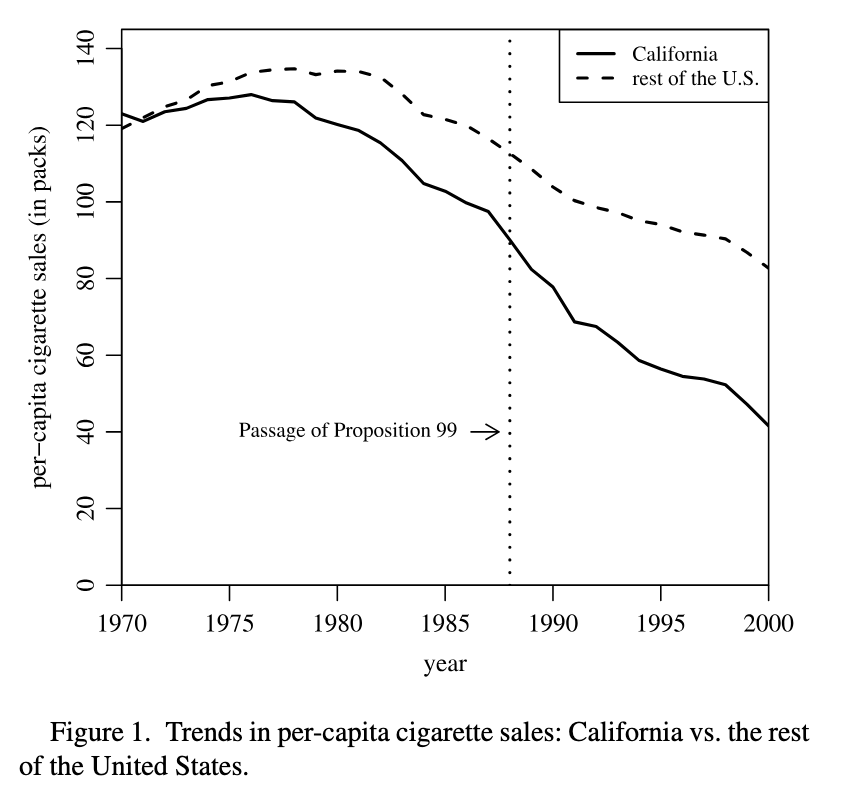
\includegraphics[scale=0.4]{img/fig1.png}
\end{figure}
The rest of the United States may not provide a suitable comparison group for California
\begin{itemize}
    \item Before the ban, cigarette consumption in California differed from the rest of the US
\end{itemize}

% trend similar in the 1970s
% peak in california when the rest of the US was still rising
% When Prop 99 was passed, cigarette consumption was 27% higher in the rest of the country than in California
\end{frame}

%%%%%%%%%%%%%%%%%%%%%%%%%%%%%%%%%%%%%%%%%%%%%%%%%%%%%%%%%%%%%%%%%%%%%%%%%%%%%%%%
\begin{frame}{Building a synthetic California}

Create a donor pool of states from which to build a synthetic California. Include all states that:
\begin{itemize}
    \item Did not adopt large-scale tobacco control programs during the sample period
    \item Did not raise cigarette taxes by 50 cents or more in the post period
\end{itemize}

Construct a synthetic California as a weighted average of potential control states
\begin{itemize}
    \item Weights should be chosen so that the resulting synthetic California best reproduces the values of a set of predictor of cigarette consumption in California before the passage of Prop 99
\end{itemize}

\end{frame}

%%%%%%%%%%%%%%%%%%%%%%%%%%%%%%%%%%%%%%%%%%%%%%%%%%%%%%%%%%%%%%%%%%%%%%%%%%%%%%%%
\begin{frame}{State weights in synthetic California}

\begin{figure}
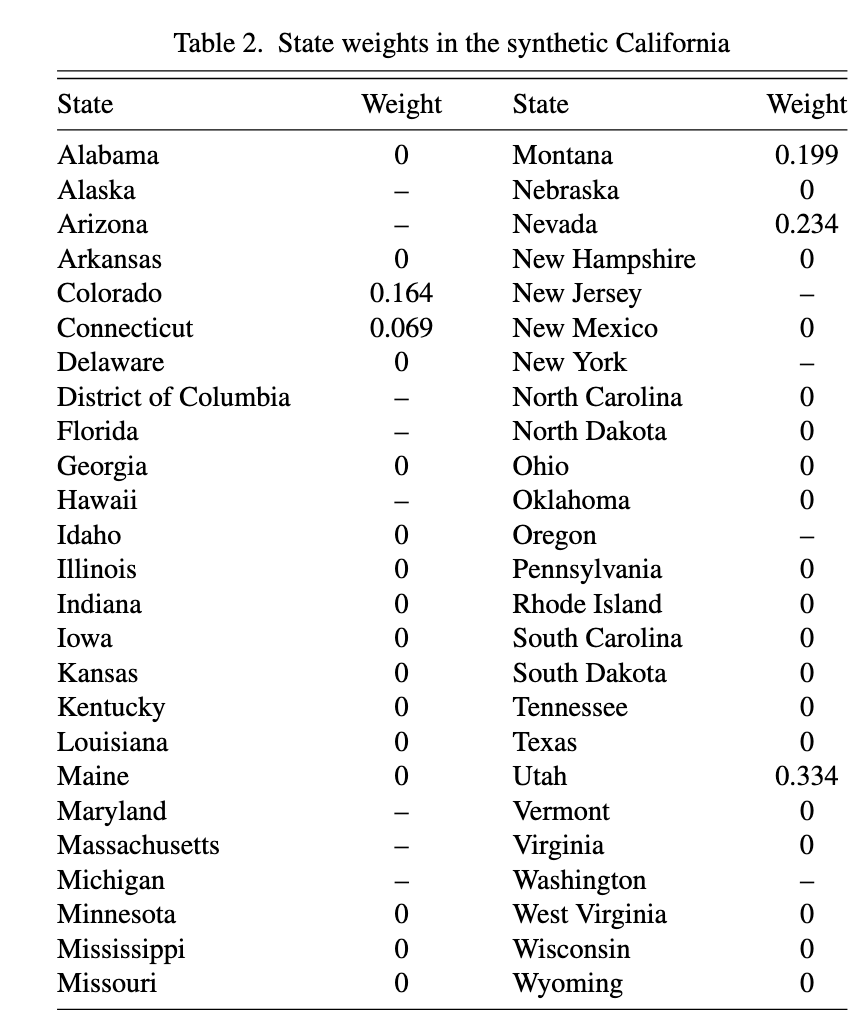
\includegraphics[scale=0.4]{img/table2.png}
\end{figure}


\end{frame}

%%%%%%%%%%%%%%%%%%%%%%%%%%%%%%%%%%%%%%%%%%%%%%%%%%%%%%%%%%%%%%%%%%%%%%%%%%%%%%%%
\begin{frame}{Cigarette sales predictor means}


\begin{figure}
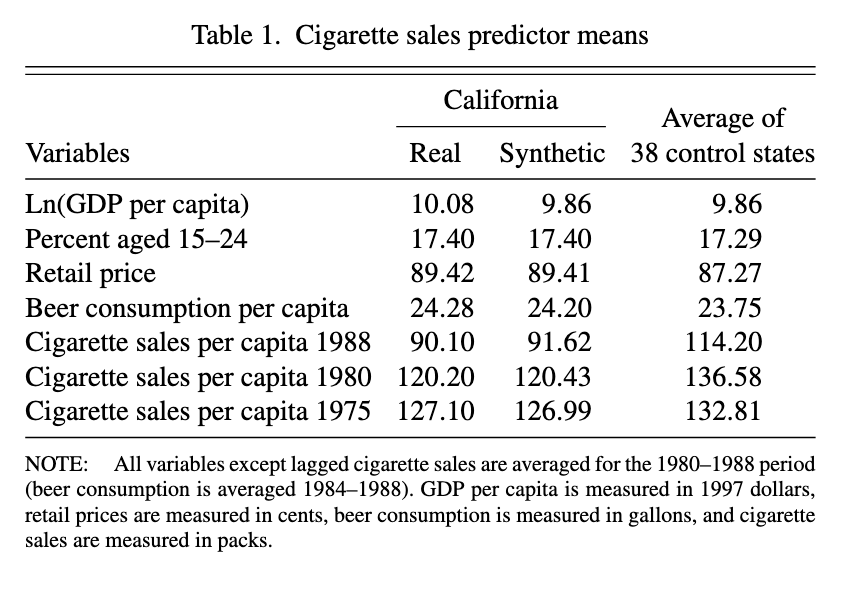
\includegraphics[scale=0.4]{img/table1.png}
\end{figure}


\end{frame}


%%%%%%%%%%%%%%%%%%%%%%%%%%%%%%%%%%%%%%%%%%%%%%%%%%%%%%%%%%%%%%%%%%%%%%%%%%%%%%%%
\begin{frame}{Synthetic California}


\begin{figure}
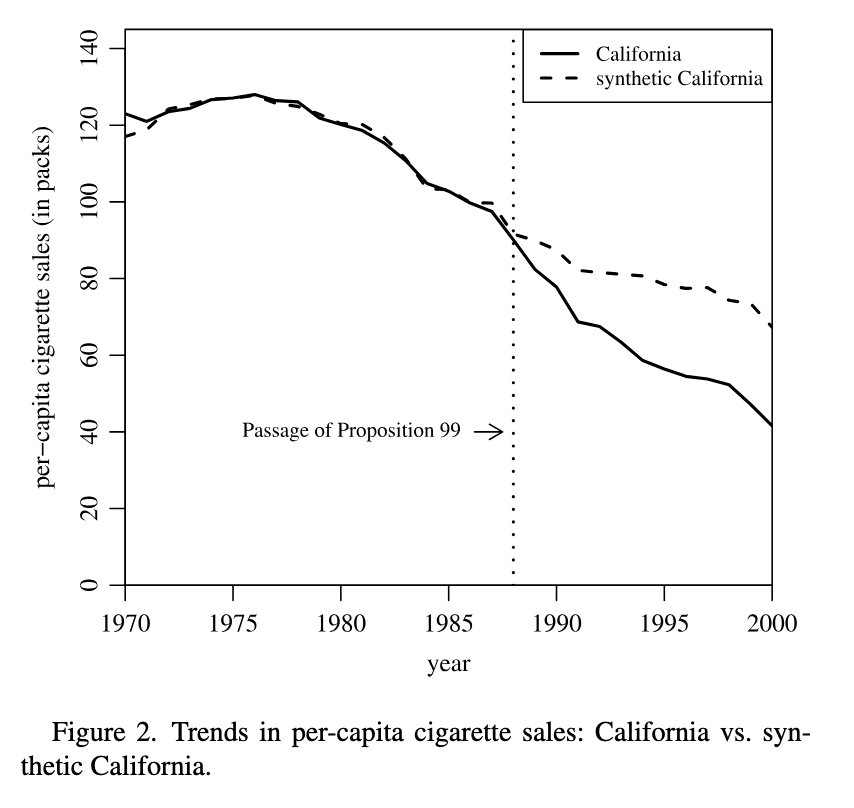
\includegraphics[scale=0.4]{img/fig2.png}
\end{figure}


\end{frame}

